\documentclass[10pt]{beamer}

\usepackage[spanish, mexico]{babel}
\usepackage[utf8]{inputenc}

\usetheme[progressbar=frametitle]{metropolis}
\usepackage{appendixnumberbeamer}

\usepackage{booktabs}
\usepackage[scale=2]{ccicons}

\usepackage{tikz}
\def\checkmark{\tikz\fill[scale=0.4](0,.35) -- (.25,0) -- (1,.7) -- (.25,.15) -- cycle;}
\usepackage{pgfplots}
\usepgfplotslibrary{dateplot}

\usepackage{xspace}
\newcommand{\themename}{\textbf{\textsc{metropolis}}\xspace}

%%
\usepackage{color}
\definecolor{lstgrey}{rgb}{0.95,0.95,0.95}
\definecolor{mygreen}{RGB}{28,172,0} % color values Red, Green, Blue
\definecolor{mylilas}{RGB}{170,55,241}

\usepackage{listings}
\lstset{language=Python,
       backgroundcolor=\color{lstgrey},
       frame=single,
       basicstyle=\footnotesize\ttfamily,
       captionpos=b,
       tabsize=2,
  }

\lstset{language=Python,%
  %basicstyle=\color{red},
  breaklines=true,%
  morekeywords={python2tikz},
  keywordstyle=\color{blue},%
  morekeywords=[2]{1}, keywordstyle=[2]{\color{black}},
  identifierstyle=\color{black},%
  stringstyle=\color{mylilas},
  commentstyle=\color{mygreen},%
  showstringspaces=false,%without this there will be a symbol in the places where there is a space
  numbers=left,%
  numberstyle={\tiny \color{black}},% size of the numbers
  numbersep=9pt, % this defines how far the numbers are from the text
  emph=[1]{for,end,break},emphstyle=[1]\color{red}, %some words to emphasise
  %emph=[2]{word1,word2}, emphstyle=[2]{style},    
}
%

\lstset{language=C,
       backgroundcolor=\color{lstgrey},
       frame=single,
       basicstyle=\footnotesize\ttfamily,
       captionpos=b,
       tabsize=2,
  }

\lstset{language=C,%
  %basicstyle=\color{red},
  breaklines=true,%
  morekeywords={c2tikz},
  keywordstyle=\color{blue},%
  morekeywords=[2]{1}, keywordstyle=[2]{\color{black}},
  identifierstyle=\color{black},%
  stringstyle=\color{mylilas},
  commentstyle=\color{mygreen},%
  showstringspaces=false,%without this there will be a symbol in the places where there is a space
  numbers=left,%
  numberstyle={\tiny \color{black}},% size of the numbers
  numbersep=9pt, % this defines how far the numbers are from the text
  emph=[1]{for,end,break},emphstyle=[1]\color{red}, %some words to emphasise
  %emph=[2]{word1,word2}, emphstyle=[2]{style},    
}
%


\title{ISI437 - Inteligencia Artificial}
\subtitle{Introducción y generalidades}
\date{\today}
% \date{}
\author{Ing. Jose Eduardo Laruta Espejo}
\institute{Universidad La Salle - Bolivia}
% \titlegraphic{\hfill
\includegraphics[height=1.5cm]{logo.pdf}}

\begin{document}

\maketitle

\begin{frame}[allowframebreaks]{Contenido}
  \setbeamertemplate{section in toc}[sections numbered]
  \tableofcontents[]
\end{frame}

%%%

\section{Agentes Planificadores}
\subsection{Agentes Reflejo}
\begin{frame}
    \frametitle{Agentes Reflejo}
    \begin{itemize}
        \item Escoge una acción basado en el estado actual percibido (tal vez incluya algo de memoria).
        \item Puede tener memoria o un modelo del entorno en el estado actual.
        \item No considera futuras consecuencias de las acciones.
        \item Considera cómo el mundo \alert{está} en un momento dado.
    \end{itemize}
    \pause
    Puede un agente reflejo ser racional?
  
\end{frame}

\begin{frame}
  \frametitle{Agentes Reflejo}
  \begin{columns}

    \begin{column}{0.4\textwidth}
      Considere a nuestro agente Pacman como un agente reflejo, la estrategia
      dicta a moverse en dirección de la comida más cercana.  
      
      ¿Se puede considerar una solución óptima?
    \end{column}
    
    \begin{column}{0.6\textwidth}
      \begin{figure}[!h] 
        \centering
        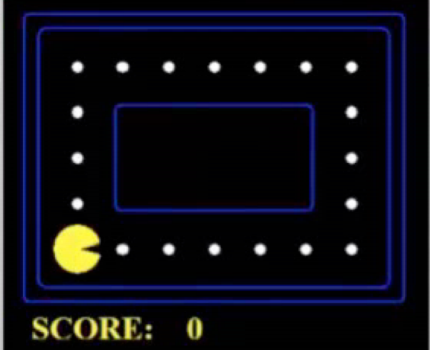
\includegraphics[width=0.7\textwidth]{img/pacman1}
      \end{figure}  
    \end{column}

  \end{columns}
\end{frame}

\begin{frame}
  \frametitle{Agentes Reflejo 2}
  \begin{columns}

    \begin{column}{0.4\textwidth}
      Considere a nuestro agente Pacman como un agente reflejo, la estrategia
      dicta a moverse en dirección de la comida más cercana.  
      
      ¿Se puede considerar una solución óptima?
    \end{column}
    
    \begin{column}{0.6\textwidth}
      \begin{figure}[!h] 
        \centering
        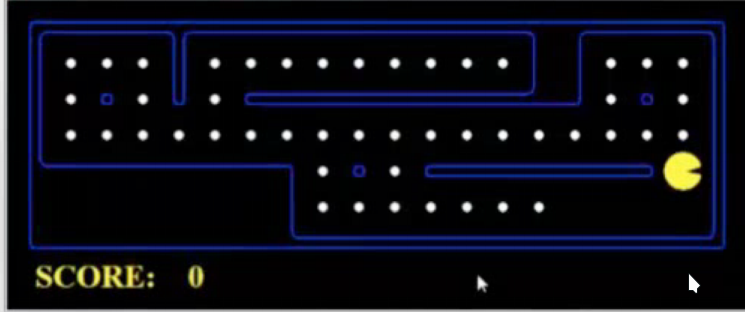
\includegraphics[width=1\textwidth]{img/pacman2}
      \end{figure}  
    \end{column}

  \end{columns}
\end{frame}

\subsection{Agentes que planifican}

\begin{frame}
  \frametitle{Agentes que planifican}
  \begin{itemize}
    \item Se hacen la pregunta ``que pasa si...''.
    \item Las decisiones se basan en las consecuencias de las acciones.
    \item Se necesita un modelo de cómo evoluciona el entorno en respuesta a las acciones.
    \item Se debe formular un \alert{objetivo}.
    \item Considera cómo el entorno \alert{podría estar}.
  \end{itemize}
\end{frame}

\begin{frame}
  \frametitle{Planeamiento Óptimo vs Completo}
  \begin{columns}
    \begin{column}{0.5\textwidth}
      \textbf{ÓPTIMO}

      Se consigue el objetivo con \alert{costo mínimo}.
    \end{column}
    \begin{column}{0.5\textwidth}
      \textbf{COMPLETO}

      Cuando existe una solución, ésta es encontrada.
    \end{column}
  \end{columns}
\end{frame}

\begin{frame}
  \frametitle{Planeamiento vs Replaneamiento}
  \begin{columns}
    \begin{column}{0.5\textwidth}
      \textbf{Planeamiento}
      
      Explora la secuencia de acciones completa y elige la mejor solución.
    \end{column}
    \begin{column}{0.5\textwidth}
      \textbf{Replaneamiento}
      
      Define una estrategia a corto plazo y cuando consigue un objetivo secundario vuelve a 
      calcular una nueva estrategia.
    \end{column}
  \end{columns}
\end{frame}

\section{Problemas de búsqueda}
\begin{frame}
  \frametitle{Problemas de búsqueda}

  Un \textbf{problema de búsqueda} consiste en:
  \begin{itemize}
    \item Un \alert{espacio de estados}.
    \item Una \alert{función sucesora}.
    \item Un estado \alert{inicial} y un \alert{objetivo}.
  \end{itemize}
  
  Una \textbf{solución} es una secuencia de acciones (un plan) que transforma el estado inicial
  en el estado objetivo.
\end{frame}

\begin{frame}
  \frametitle{Espacio de estados}
  El \textbf{espacio de estados} es el conjunto de todas las posibles configuraciones del problema.

  \begin{figure}[!h] 
    \centering
    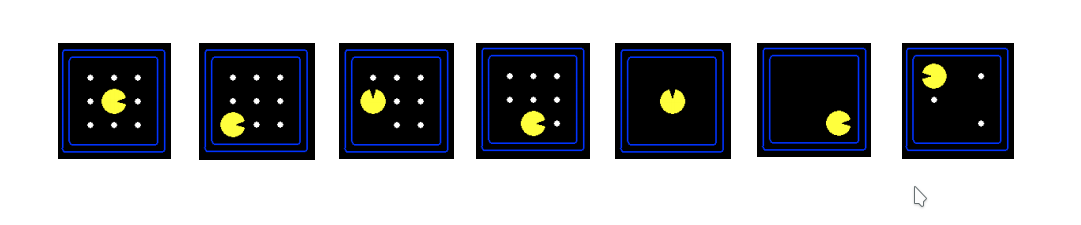
\includegraphics[width=1\textwidth]{img/state_space}
  \end{figure} 

\end{frame}

\begin{frame}
  \frametitle{Función sucesora}
  La \textbf{función sucesora} define cuáles son las acciones disponibles para un estado dado y 
  cuáles los estados consecuencia para dichas acciones.

  \begin{figure}[!h] 
    \centering
    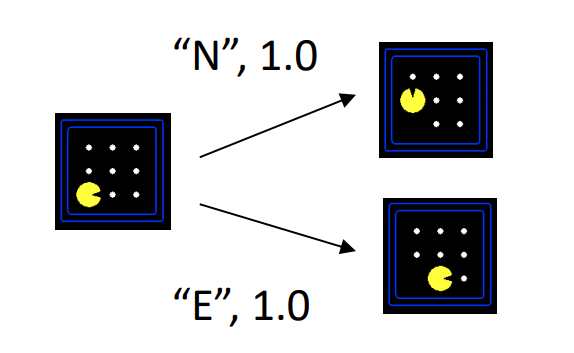
\includegraphics[width=0.5\textwidth]{img/sucesora}
  \end{figure} 

\end{frame}


{\setbeamercolor{palette primary}{fg=black, bg=yellow}
\begin{frame}[standout]
  Ejemplo
\end{frame}
}

\begin{frame}
  \frametitle{Ejemplo: Viajando por Rumania}

  \begin{figure}[!h] 
    \centering
    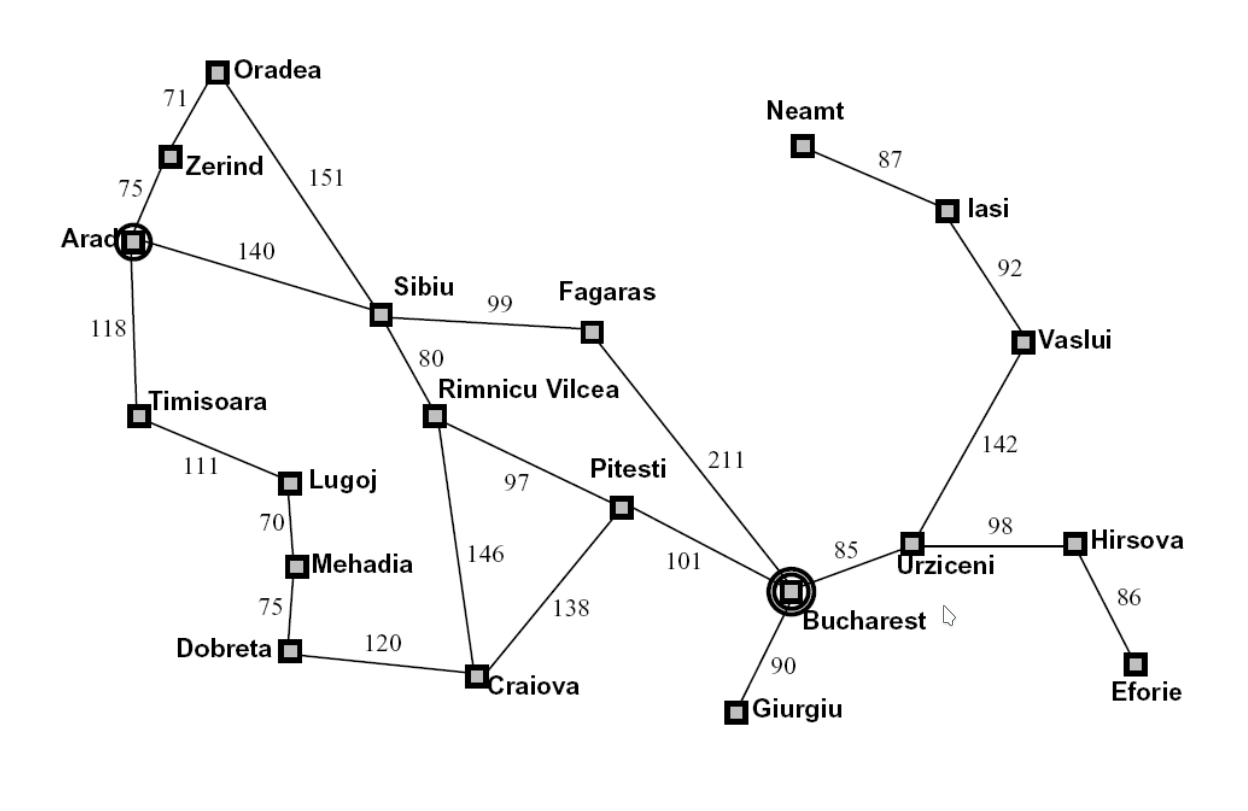
\includegraphics[width=\textwidth]{img/rumania}
  \end{figure} 
  
\end{frame}

\begin{frame}
  \frametitle{Ejemplo: Viajando por Rumania}

\begin{itemize}
  \item \textbf{Espacio de estados:} Ciudades
  \item \textbf{Función sucesora:} Carreteras, viaje a una ciudad adyacente con $costo=distancia$.
  \item \textbf{Estado Inicial:} Arad
  \item \textbf{Estado objetivo:} $estado == Bucharest?$.
  \item \textbf{Solución}
\end{itemize}
  
\end{frame}

\begin{frame}
  \frametitle{Ejemplo: Pacman}

  El estado del mundo incluye todos los detalles del entorno. 
  \begin{figure}[!h] 
    \centering
    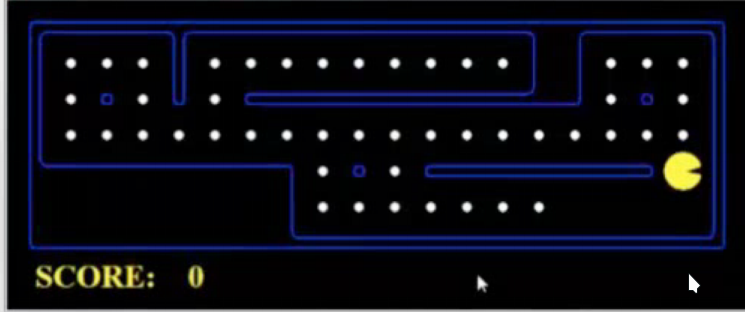
\includegraphics[width=\textwidth]{img/pacman2}
  \end{figure} 
  
\end{frame}

\begin{frame}
  \frametitle{Ejemplo: Pacman}

  \begin{columns}
    \begin{column}{0.5\textwidth}
      Problema: \textbf{Recorrido}
      \begin{itemize}
        \item Estados:
        \item Acciones:
        \item F. Sucesora:
        \item Objetivo:
      \end{itemize}
    \end{column}
    
    \begin{column}{0.5\textwidth}
      \begin{figure}[!h] 
        \centering
        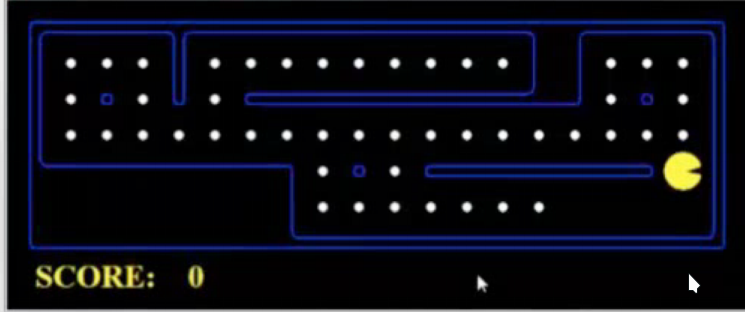
\includegraphics[width=\textwidth]{img/pacman2}
      \end{figure} 
    \end{column}
  \end{columns}

\end{frame}

\begin{frame}
  \frametitle{Ejemplo: Pacman}

  \begin{columns}
    \begin{column}{0.5\textwidth}
      Problema: \textbf{Acabar toda la comida}
      \begin{itemize}
        \item Estados:
        \item Acciones:
        \item F. Sucesora:
        \item Objetivo:
      \end{itemize}
    \end{column}
    
    \begin{column}{0.5\textwidth}
      \begin{figure}[!h] 
        \centering
        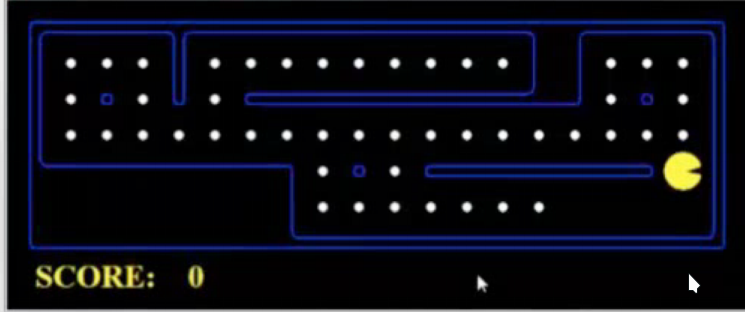
\includegraphics[width=\textwidth]{img/pacman2}
      \end{figure} 
    \end{column}
  \end{columns}

\end{frame}

\begin{frame}
  \frametitle{Dimensión del espacio de estados}
  \begin{columns}
    \begin{column}{0.5\textwidth}
      \begin{itemize}
        \item Estado del mundo:
          \begin{itemize}
            \item Posiciones del agente: 120
            \item Cantidad de puntos: 30
            \item Posiciones de fantasmas: 12
            \item Orientacion del agente: NSEW
          \end{itemize}
        
        \item Cantidad:
          \begin{itemize}
            \item Mundo: $120 \times (2^30) \times (12^2) \times 4$
            \item Estados para recorrido: $120$
            \item Estados para comer: $120 \times 2^30$
          \end{itemize}
      \end{itemize}  
    \end{column}

    \begin{column}{0.5\textwidth}
      
      \begin{figure}[!h] 
        \centering
        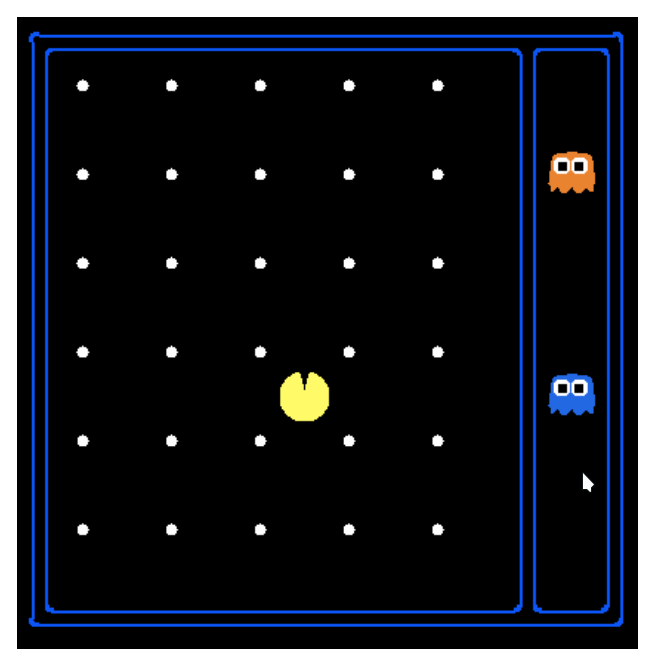
\includegraphics[width=\textwidth]{img/estados}
      \end{figure} 

    \end{column}    
  \end{columns}

\end{frame}


\begin{frame}
  \frametitle{Ejercicio}

  \begin{figure}[!h] 
    \centering
    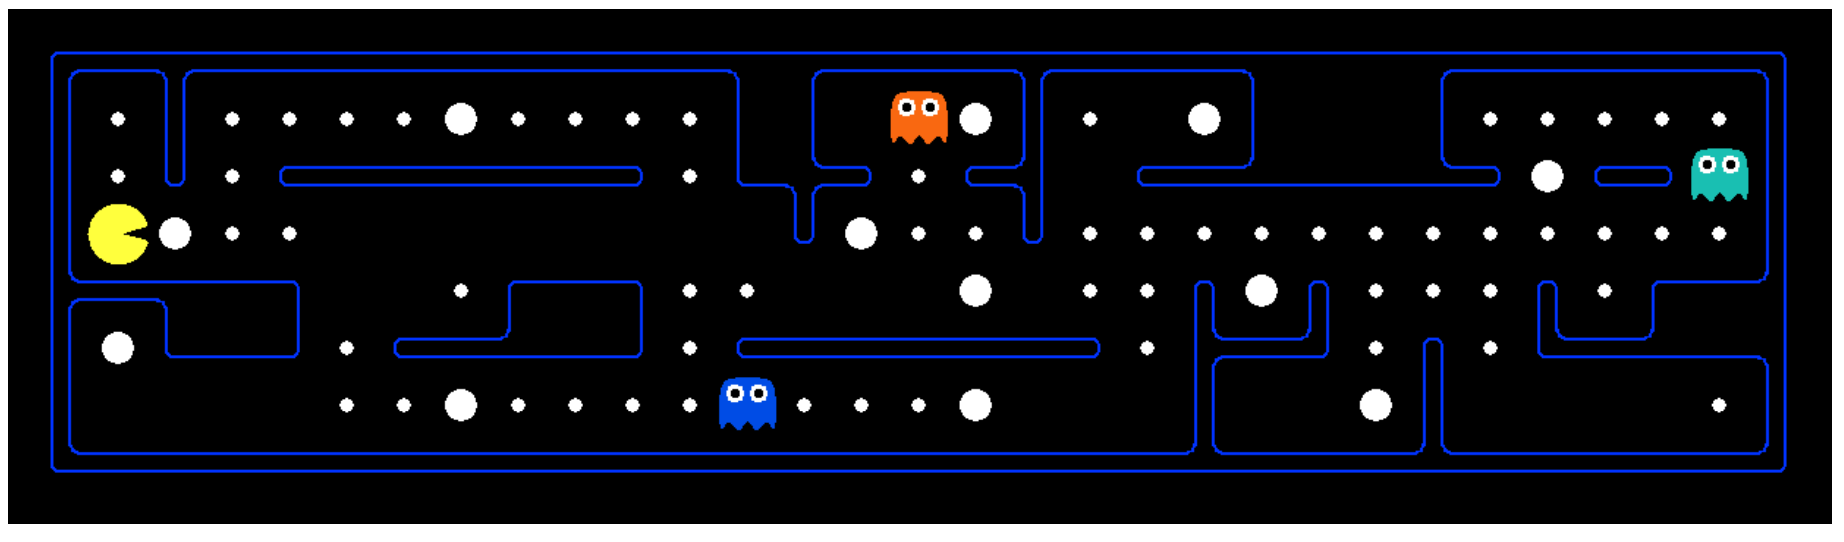
\includegraphics[width=\textwidth]{img/completo1}
  \end{figure}
  \textbf{Problema:} Comer todos los puntos mientras se mantiene a los fantasmas asustados.
  \pause
  \begin{itemize}
    \item Posición, puntos, puntos de poder, tiempo restante
  \end{itemize}
\end{frame}


\subsection{Grafos de Espacio de estado}

\begin{frame}
  \frametitle{Grafos de Espacio de estado}

  \begin{figure}[!h] 
    \centering
    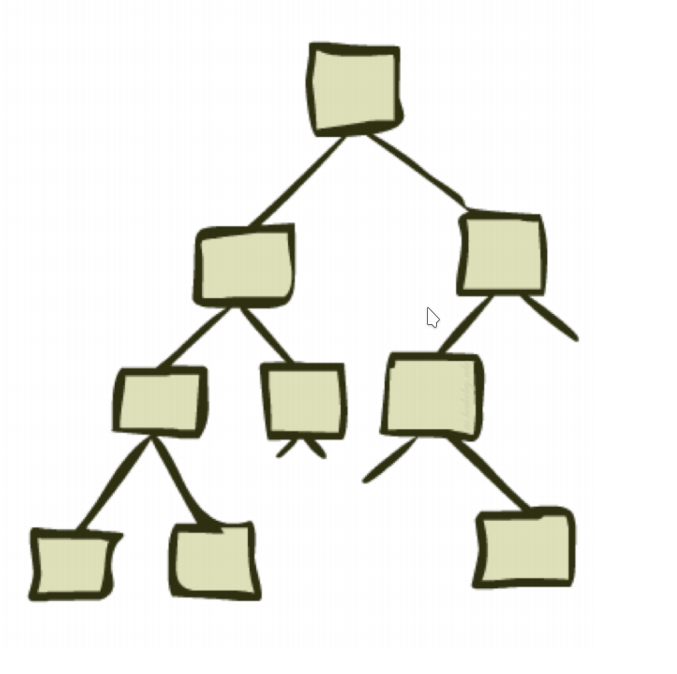
\includegraphics[width=0.5\textwidth]{img/grafo1}
  \end{figure}

\end{frame}

\begin{frame}
  \frametitle{Grafos de Espacio de estado}
  \begin{columns}
    \begin{column}{0.5\textwidth}
      \begin{itemize}
        \item Representación matemática:
          \begin{itemize}
            \item Los nodos son configuraciones abstractas.
            \item Los arcos representan sucesores (resultados de acciones).
            \item El objetivo es un conjunto de nodos objetivo (o uno solo).
          \end{itemize}
        \item Cada estado solamente ocurre una vez.
        \item Es dificil construir este grafo completo en la memoria.
      \end{itemize}
    \end{column}
    \begin{column}{0.5\textwidth}
      \begin{figure}[!h] 
        \centering
        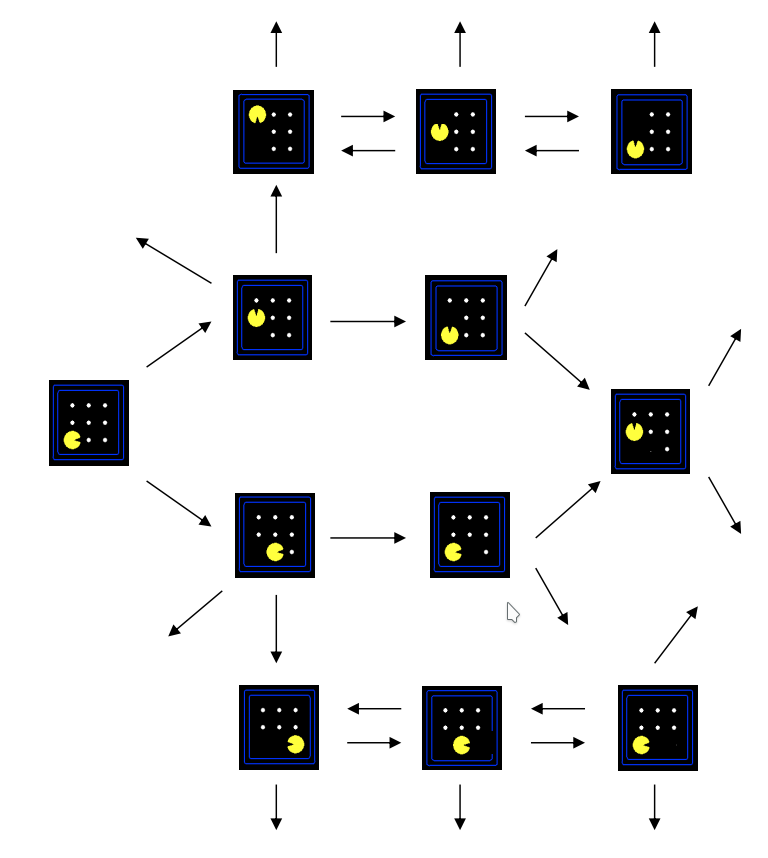
\includegraphics[width=\textwidth]{img/grafo2}
      \end{figure}
    \end{column}
  \end{columns}
\end{frame}

\begin{frame}
  \frametitle{Grafos de Espacio de estado}
  \begin{columns}
    \begin{column}{0.5\textwidth}
      \begin{itemize}
        \item Representación matemática:
          \begin{itemize}
            \item Los nodos son configuraciones abstractas.
            \item Los arcos representan sucesores (resultados de acciones).
            \item El objetivo es un conjunto de nodos objetivo (o uno solo).
          \end{itemize}
        \item Cada estado solamente ocurre una vez.
        \item Es dificil construir este grafo completo en la memoria.
      \end{itemize}
    \end{column}
    \begin{column}{0.5\textwidth}
      \begin{figure}[!h] 
        \centering
        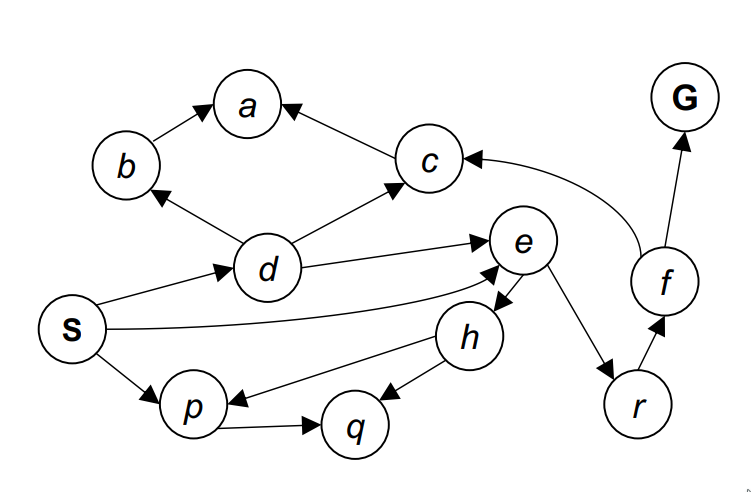
\includegraphics[width=\textwidth]{img/grafo3}
      \end{figure}
    \end{column}
  \end{columns}
\end{frame}


\subsection{Árboles de búsqueda}

\begin{frame}
  \frametitle{Árboles de búsqueda}
  \begin{figure}[!h] 
    \centering
    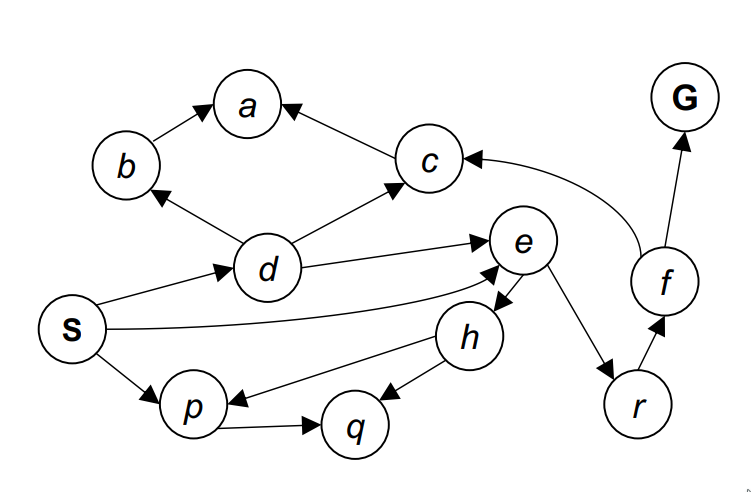
\includegraphics[width=0.5\textwidth]{img/grafo3}
  \end{figure}
  
  Un árbol de búsqueda:
  \begin{itemize}
    \item Representa el ``qué pasa si...' de los planes y sus resultados.
    \item El nodo inicial es el nodo raíz.
    \item Los nodos hijos corresponden a los sucesores.
    \item Los nodos muestran estados pero corresponden a \alert{planes}.
    \item En la práctica no se construyen los árboles completos.
  \end{itemize}

\end{frame}

\begin{frame}
  \frametitle{Árboles de búsqueda}
  \begin{figure}[!h] 
    \centering
    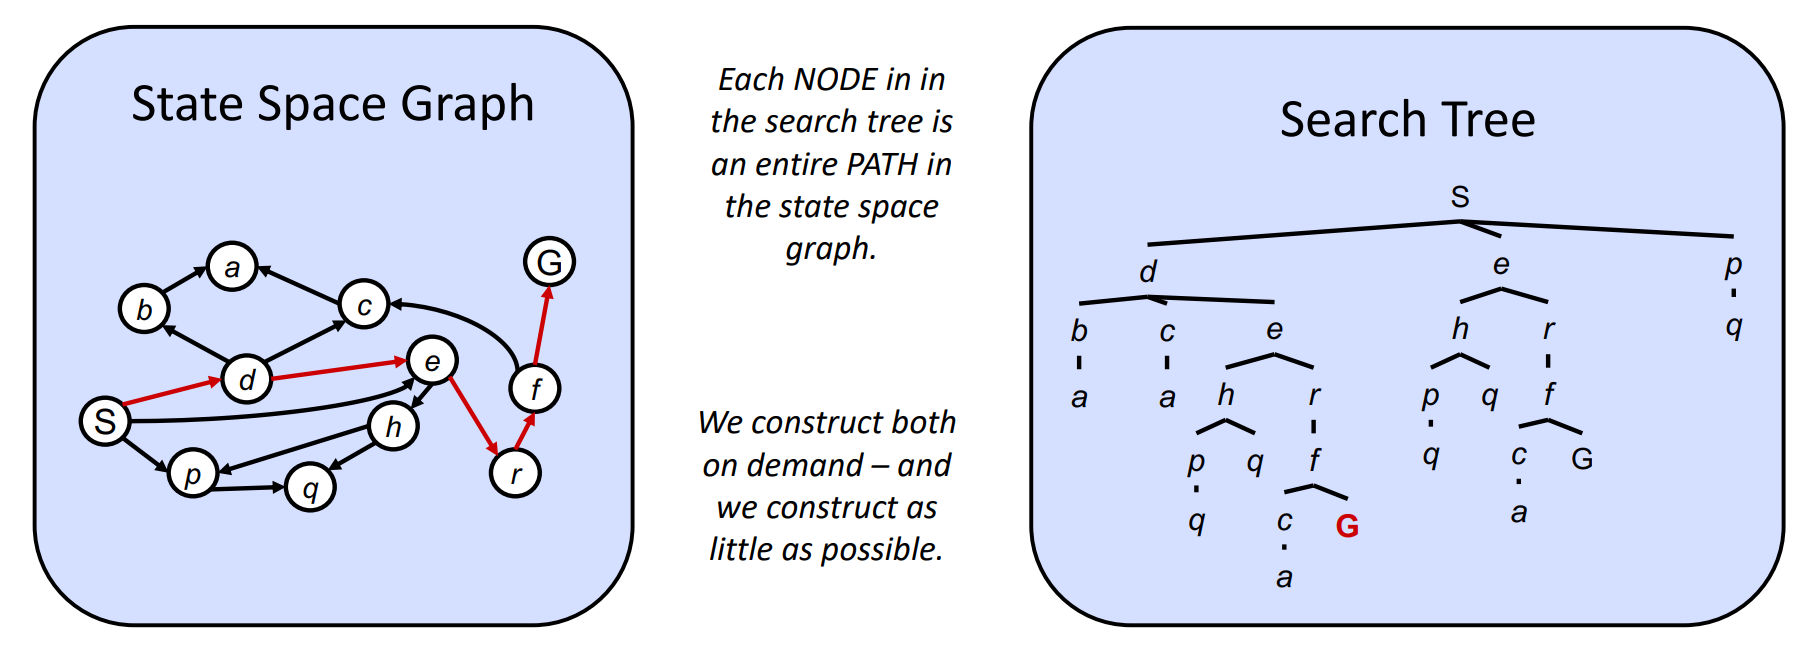
\includegraphics[width=1\textwidth]{img/spacetree}
  \end{figure}
\end{frame}

\begin{frame}
  \frametitle{Ejercicio: Árboles de búsqueda}
  \begin{figure}[!h] 
    \centering
    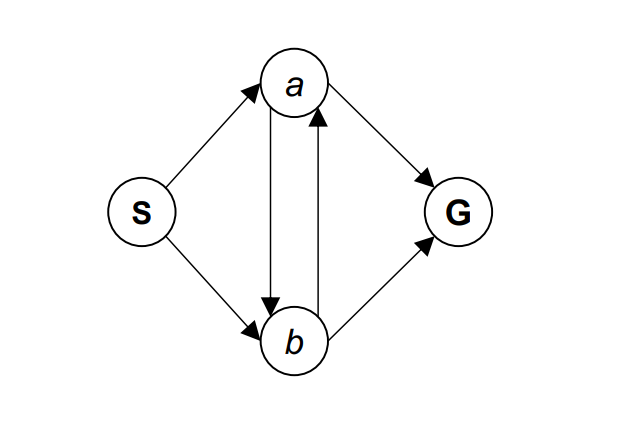
\includegraphics[width=0.7\textwidth]{img/estado2}
  \end{figure}
  Qué tan grande es el árbol de búsqueda?
  \pause
  $$ \infty $$
\end{frame}

\begin{frame}
  \frametitle{Ejemplo: Viajando por Rumania}

  \begin{figure}[!h] 
    \centering
    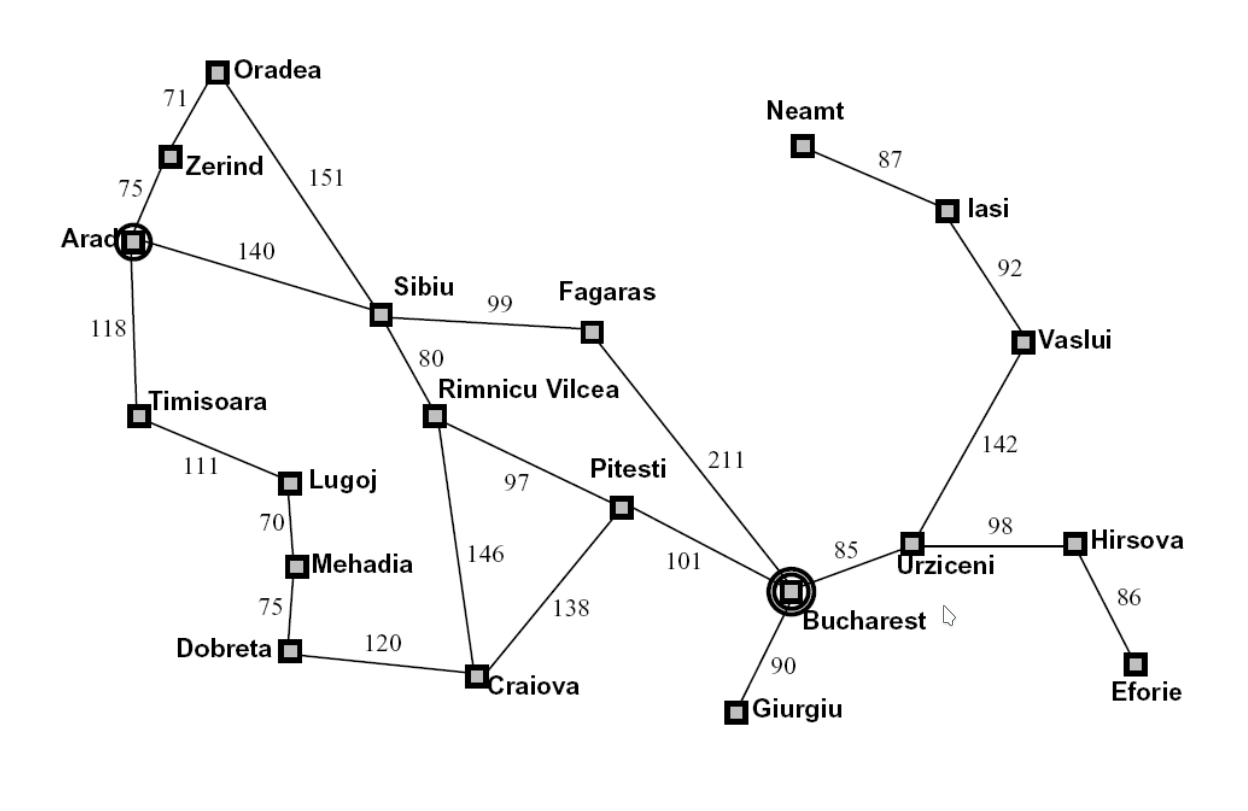
\includegraphics[width=\textwidth]{img/rumania}
  \end{figure} 
  
\end{frame}

\begin{frame}
  \frametitle{Búsqueda de árboles}

  \begin{figure}[!h] 
    \centering
    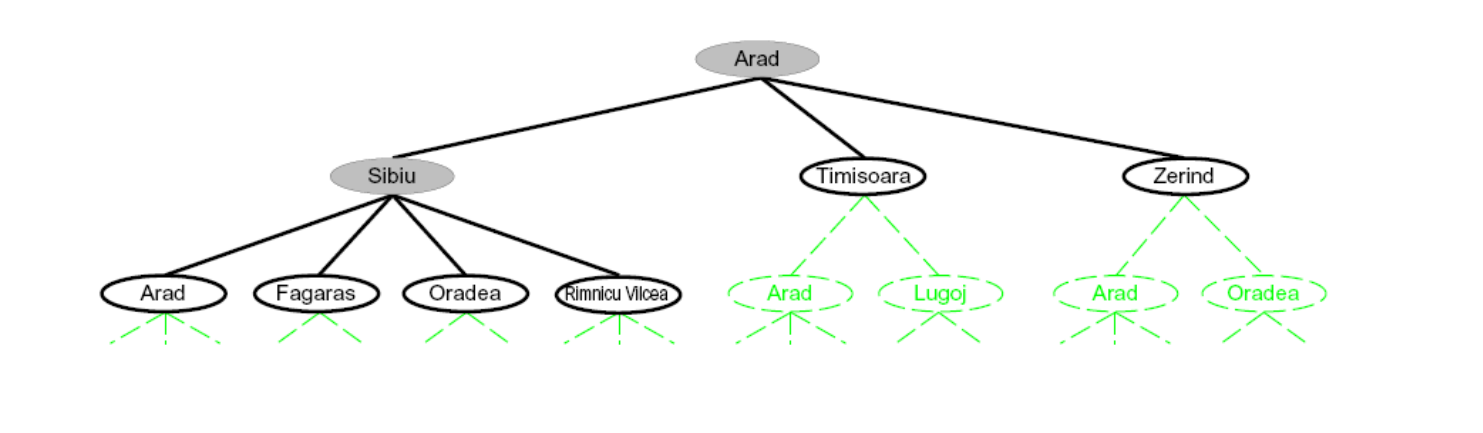
\includegraphics[width=\textwidth]{img/arbol2}
  \end{figure} 
  
  Búsqueda:
  \begin{itemize}
    \item Expandir planes potenciales.
    \item Mantener una \alert{frontera} de planes parciales bajo consideración.
    \item Tratar de expandir la \alert{menor cantidad} de nodos posible.
  \end{itemize}
\end{frame}

\begin{frame}[fragile]
  \frametitle{Búsqueda de árboles generalizada}

 \begin{lstlisting}
   def busqueda_arbol(problema, estrategia):
      inicializa el arbol con el estado inicial.
      while True:
        if no hay candidatos para expandir: 
          return falla
        seleccionar nodo para expandir
        if nodo es objetivo:
          return solucion
        else:
          expandir nodo y agregar nodos resultantes al arbol.
 \end{lstlisting}
Ideas importantes:
\begin{itemize}
  \item Frontera (fringe).
  \item Expansión de nodos.
  \item Extrategia de expansión.
\end{itemize}
\pause
\textbf{Pregunta principal:} Cuáles nodos de la frontera expandir?
\end{frame}

\begin{frame}
  \frametitle{Ejemplo: Búsqueda de árboles}

  \begin{figure}[!h] 
    \centering
    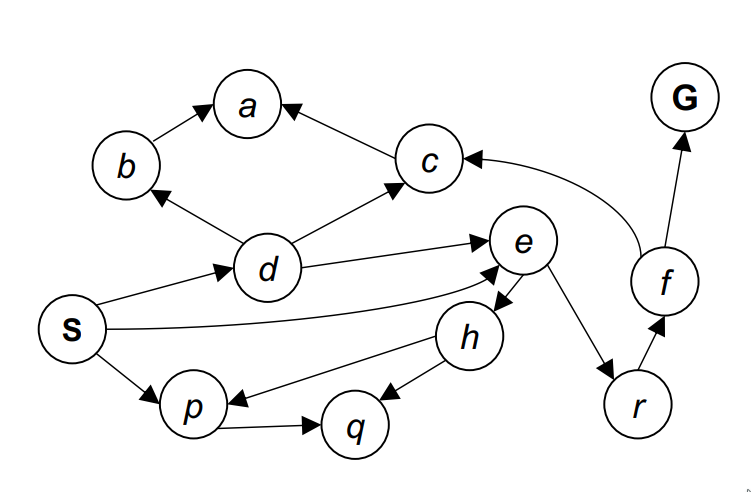
\includegraphics[width=0.75\textwidth]{img/grafo3}
  \end{figure} 

\end{frame}

\section{Búsqueda a Ciegas}

\subsection{Depth-First Search}
\begin{frame}
  \frametitle{Depth-First Search}

  \textbf{Estrategia:} Expandir el nodo con más \alert{profundidad} primero.
  \textbf{Implementación:} La frontera es una \alert{pila} (LIFO).

\end{frame}

\begin{frame}
  \frametitle{Propiedades de algoritmos de búsqueda}
  \begin{columns}
    \begin{column}{0.5\textwidth}
      \begin{itemize}
        \item Completo: Solución garantizada si existe?
        \item Óptimo: Garantizada la mejor solución?
        \item Complejidad en tiempo?
        \item Complejidad en espacio?
        \item Gráfico:
          \begin{itemize}
            \item $b$ es el factor de ramificación.
            \item $m$ es la profundidad máxima.
            \item existen soluciones en distintas profundidades.
          \end{itemize}
        \item Número de nodos en el árbol: $1 + b + b^2 + \dots + b^m = O(b^m)$
      \end{itemize}
    \end{column}
    \begin{column}{0.5\textwidth}
      \begin{figure}[!h] 
        \centering
        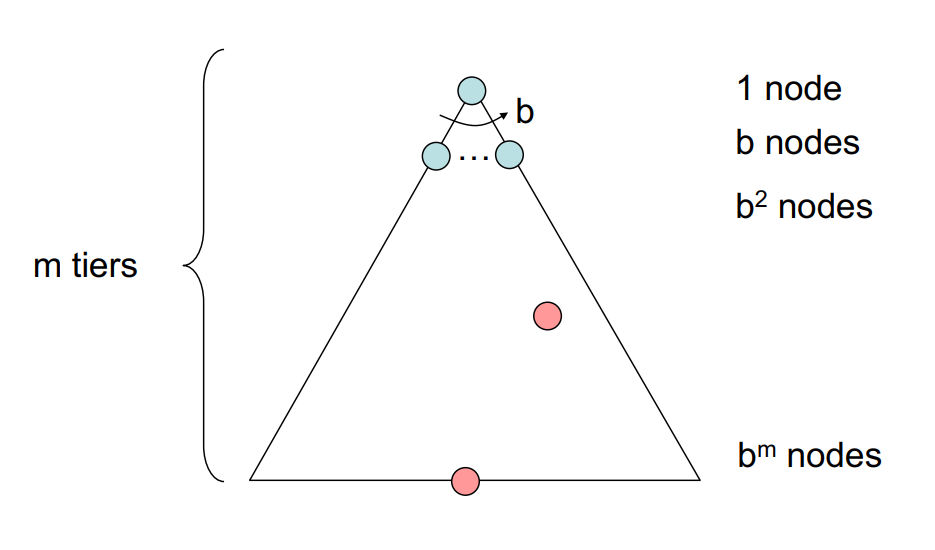
\includegraphics[width=1\textwidth]{img/dfs1}
      \end{figure} 
    \end{column}
  \end{columns}
\end{frame}


\begin{frame}
  \frametitle{Depth-First Search: propiedades}
  \begin{columns}
    \begin{column}{0.5\textwidth}
      \begin{itemize}
        \item Cuáles nodos expande DFS?
          \begin{itemize}
            \item Estrategia a la izquierda.
            \item Puede procesar todo el árbol.
            \item Si el arbol es finito, toma $O(b^m)$.
          \end{itemize}
        \item Cuánto espacio ocupa la frontera?
          \begin{itemize}
            \item .
          \end{itemize}
        \item Es completo?
          \begin{itemize}
            \item .
          \end{itemize}
        \item Es óptimo?
          \begin{itemize}
            \item .
          \end{itemize}
      \end{itemize}
    \end{column}
    \begin{column}{0.5\textwidth}
      \begin{figure}[!h] 
        \centering
        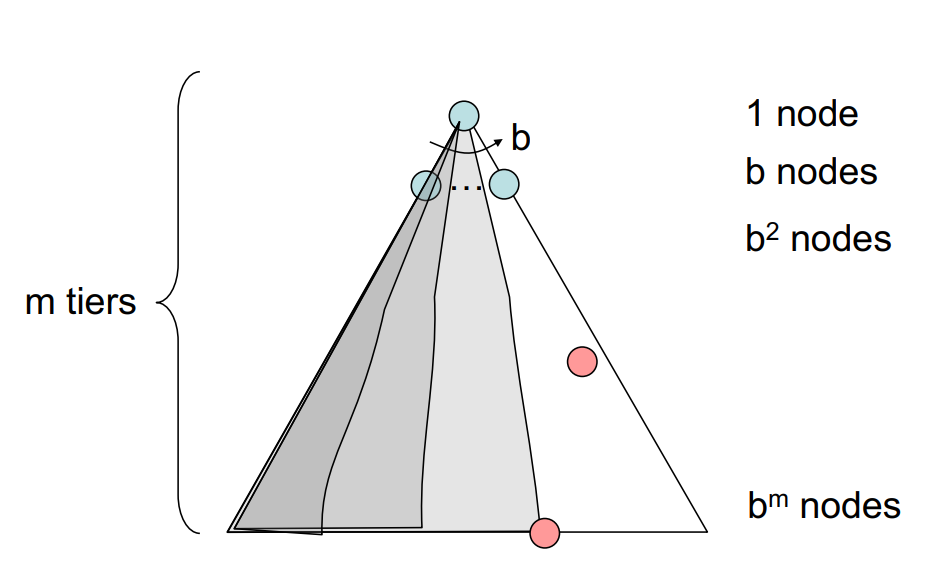
\includegraphics[width=1\textwidth]{img/dfs2}
      \end{figure} 
    \end{column}
  \end{columns}
\end{frame}

\begin{frame}
  \frametitle{Depth-First Search: propiedades}
  \begin{columns}
    \begin{column}{0.5\textwidth}
      \begin{itemize}
        \item Cuáles nodos expande DFS?
          \begin{itemize}
            \item Estrategia a la izquierda.
            \item Puede procesar todo el árbol.
            \item Si el arbol es finito, toma $O(b^m)$.
          \end{itemize}
        \item Cuánto espacio ocupa la frontera?
          \begin{itemize}
            \item Solamente los hijos en el camino principal $O(bm)$.
          \end{itemize}
        \item Es completo?
          \begin{itemize}
            \item $m$ puede ser infinito, solo si evitamos ciclos.
          \end{itemize}
        \item Es óptimo?
          \begin{itemize}
            \item No, encuentra la solución más cercana a la izquierda, sin 
            importar profundidad ni costo.
          \end{itemize}
      \end{itemize}
    \end{column}
    \begin{column}{0.5\textwidth}
      \begin{figure}[!h] 
        \centering
        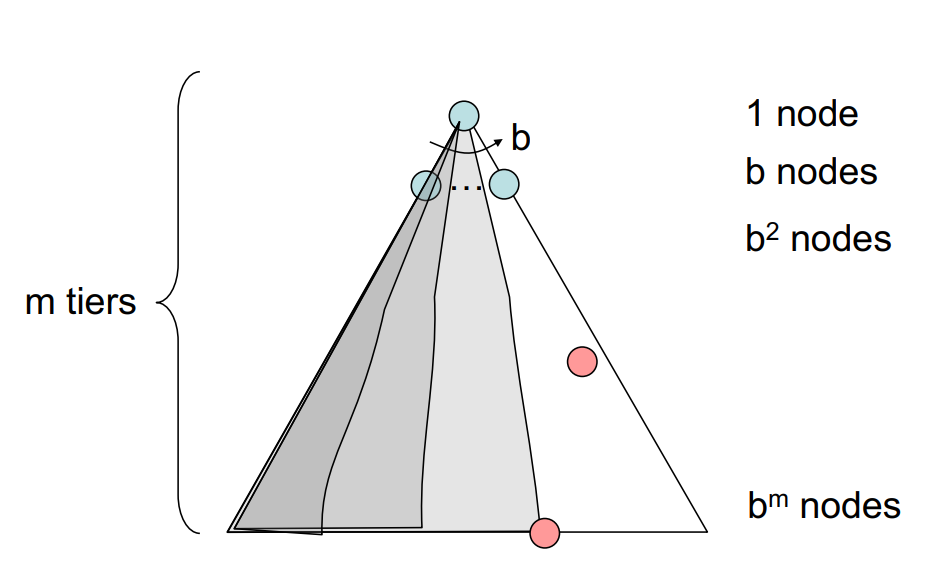
\includegraphics[width=1\textwidth]{img/dfs2}
      \end{figure} 
    \end{column}
  \end{columns}
\end{frame}

\subsection{Breadth-First Search}

\begin{frame}
  \frametitle{Breadth-First Search}

  \textbf{Estrategia:} Expandir el nodo con menos \alert{profundidad} primero.
  \textbf{Implementación:} La frontera es una \alert{cola} (FIFO).

\end{frame}

\begin{frame}
  \frametitle{Breadth-First Search: propiedades}
  \begin{columns}
    \begin{column}{0.5\textwidth}
      \begin{itemize}
        \item Cuáles nodos expande BFS?
          \begin{itemize}
            \item Los nodos más cercanos.
            \item $s$ es la profundidad de la solución más cercana.
            \item La búsqueda toma $O(b^s)$ en tiempo.
          \end{itemize}
        \item Cuánto espacio ocupa la frontera?
          \begin{itemize}
            \item Aproximadamente el nivel final $O(b^s)$.
          \end{itemize}
        \item Es completo?
          \begin{itemize}
            \item $s$ debe ser finito si existe una solución, entonces si.
          \end{itemize}
        \item Es óptimo?
          \begin{itemize}
            \item Solamente si todos los costos son 1.
          \end{itemize}
      \end{itemize}
    \end{column}
    \begin{column}{0.5\textwidth}
      \begin{figure}[!h] 
        \centering
        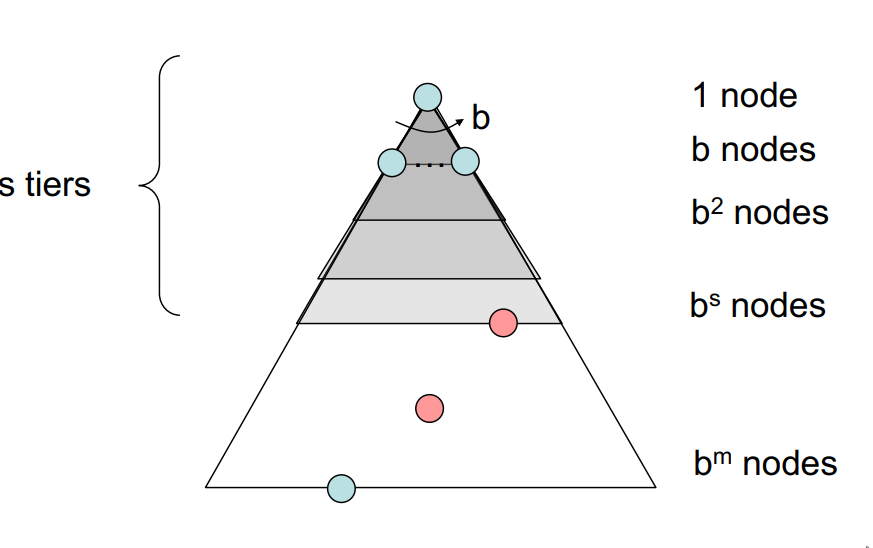
\includegraphics[width=1\textwidth]{img/bfs1}
      \end{figure} 
    \end{column}
  \end{columns}
\end{frame}

\begin{frame}
  \frametitle{Quiz: DFS vs BFS}

  \begin{itemize}
    \item Cuándo BFS es mejor que DFS?
      \begin{itemize}
        \item Encuentra el camino más corto.
      \end{itemize}
    \item Cuándo DFS es mejor que BFS?
      \begin{itemize}
        \item Mejor aprovechamiento de la memoria.
      \end{itemize}
  \end{itemize}
  
\end{frame}

\begin{frame}
  \frametitle{Iterative Deepening}
  
  \begin{columns}
    \begin{column}{0.5\textwidth}
      \begin{itemize}
        \item Idea: aprovechar memoria usada por DFS con el tiempo y la solución corta de BFS.
          \begin{itemize}
            \item Corre DFS con límite de profundidad 1, si no hay solución\dots
            \item Corre DFS con límite de profundidad 2, si no hay solución\dots
            \item Corre DFS con límite de profundidad 3\dots
          \end{itemize}
        \item No es redundante?
          \begin{itemize}
            \item Generalmente, la mayor parte del trabajo ocurre en el nivel más bajo.
          \end{itemize}
      \end{itemize}
    \end{column}

    \begin{column}{0.5\textwidth}
      \begin{figure}[!h] 
        \centering
        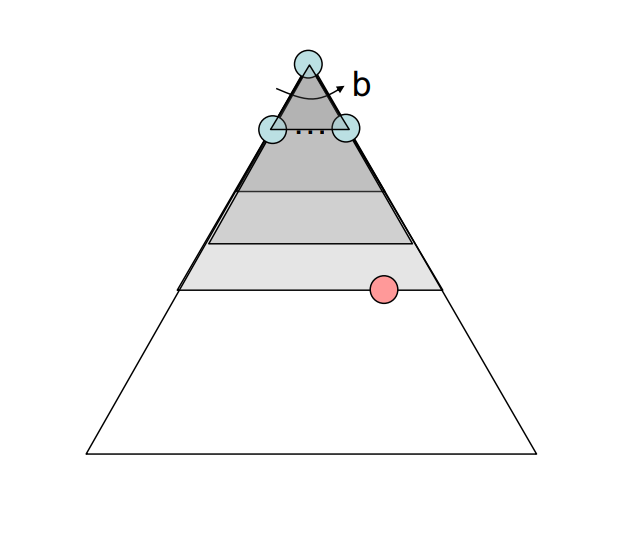
\includegraphics[width=1\textwidth]{img/iter}
      \end{figure} 
    \end{column}
  \end{columns}

\end{frame}

\subsection{Cost-sensitive search}

\begin{frame}
  \frametitle{Cost-sensitive search}

  \begin{figure}[!h] 
    \centering
    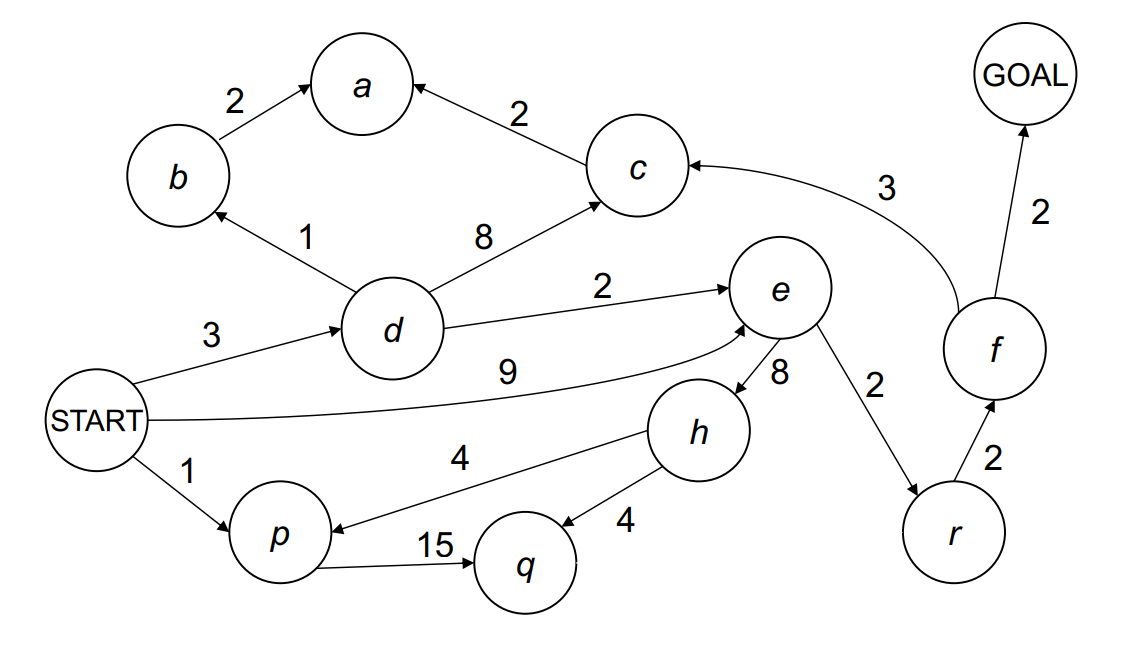
\includegraphics[width=1\textwidth]{img/ucs1}
  \end{figure} 

  BFS encuentra el mejor camino en términos de números de acciones.
  No encuentra el camino con el menor costo. Ahora trataremos 
  un algoritmo similar que encuentra el camino con el menor costo.
  
\end{frame}
\subsection{Uniform-Cost Search}

\begin{frame}
  \frametitle{Uniform-Cost Search}

  \textbf{Estrategia:} Expandir el nodo con menos \alert{costo} primero.
  \textbf{Implementación:} La frontera es una \alert{cola de prioritaria} (costo acumulado).

\end{frame}

\begin{frame}
  \frametitle{Uniform Cost Search: propiedades}
  \begin{columns}
    \begin{column}{0.6\textwidth}
      \begin{itemize}
        \item Cuáles nodos expande UCS?
          \begin{itemize}
            \item Todos los nodos con costo $<$ solución más barata.
            \item Si el costo de la solución es $C^*$ y los arcos al menos $\epsilon$, entonces,
            la ``profundidad efectiva'' es aprox. $\frac{C^*}{\epsilon}$.
            \item La búsqueda toma $O(b^{\frac{C^*}{\epsilon}})$ en tiempo.
          \end{itemize}
        \item Cuánto espacio ocupa la frontera?
          \begin{itemize}
            \item Aproximadamente el nivel final $O(b^{\frac{C^*}{\epsilon}})$.
          \end{itemize}
        \item Es completo?
          \begin{itemize}
            \item Asumiendo que la mejor solución tiene costo finito.
          \end{itemize}
        \item Es óptimo?
          \begin{itemize}
            \item Si.
          \end{itemize}
      \end{itemize}
    \end{column}
    \begin{column}{0.4\textwidth}
      \begin{figure}[!h] 
        \centering
        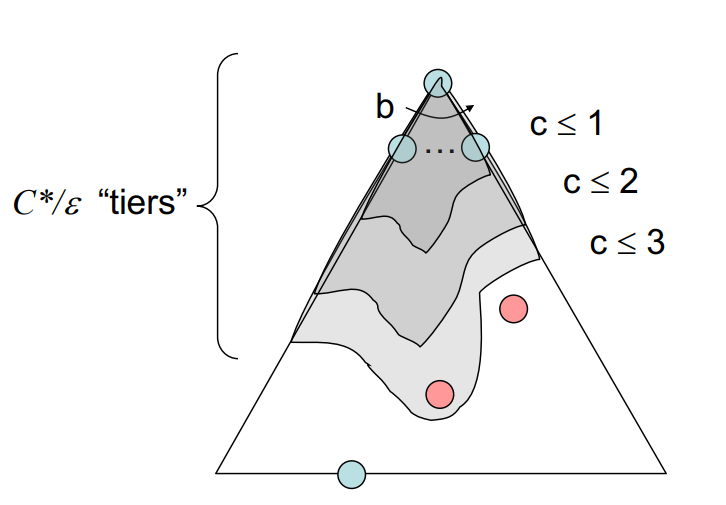
\includegraphics[width=1\textwidth]{img/ucs2}
      \end{figure} 
    \end{column}
  \end{columns}
\end{frame}

\begin{frame}
  \frametitle{Uniform Cost: Detalles}

  \begin{itemize}
    \item UCS explora contornos de costo creciente.
    \item UCS es completo y óptimo.
    \item Lo malo:
      \begin{itemize}
        \item Explora opciones en ``todas las direcciones''.
        \item No existe información acerca de la ubicación del objetivo.
      \end{itemize}
  \end{itemize}
  
\end{frame}

\subsection{Implementación}
\begin{frame}
  \frametitle{La única cola}

  \begin{itemize}
    \item Todos estos algoritmos son iguales excepto por la estrategia de expansión de la \alert{frontera}
      \begin{itemize}
        \item Conceptualmente, todas las fronteras son colas prioritarias.
        \item En la práctica, para DFS y BFS, se puede implementar usando pilas y colas tradicionales.
        \item Se puede programar una implementación que tome como variable el objeto de cola.
      \end{itemize}
  \end{itemize}

\end{frame}

\begin{frame}
  \frametitle{Búsqueda y modelos}

  \begin{itemize}
    \item Los algoritmos de búsqueda operan sobre modelos del entorno.
      \begin{itemize}
        \item El agente no prueba todas las posibilidades en el mundo real.
        \item La planificación se hace en \textit{simulación}.
        \item La búsqueda es tan buena como el modelo.
      \end{itemize}
  \end{itemize}

\end{frame}
{\setbeamercolor{palette primary}{fg=black, bg=yellow}
\begin{frame}[standout]
  Preguntas?
\end{frame}
}

\appendix

% \begin{frame}[fragile]{Backup slides}
%   Sometimes, it is useful to add slides at the end of your presentation to
%   refer to during audience questions.

%   The best way to do this is to include the \verb|appendixnumberbeamer|
%   package in your preamble and call \verb|\appendix| before your backup slides.

%   \themename will automatically turn off slide numbering and progress bars for
%   slides in the appendix.
% \end{frame}

% \begin{frame}[allowframebreaks]{Referencias}
% .
% \end{frame}

\end{document}
